\begin{figure}[H]
\centering
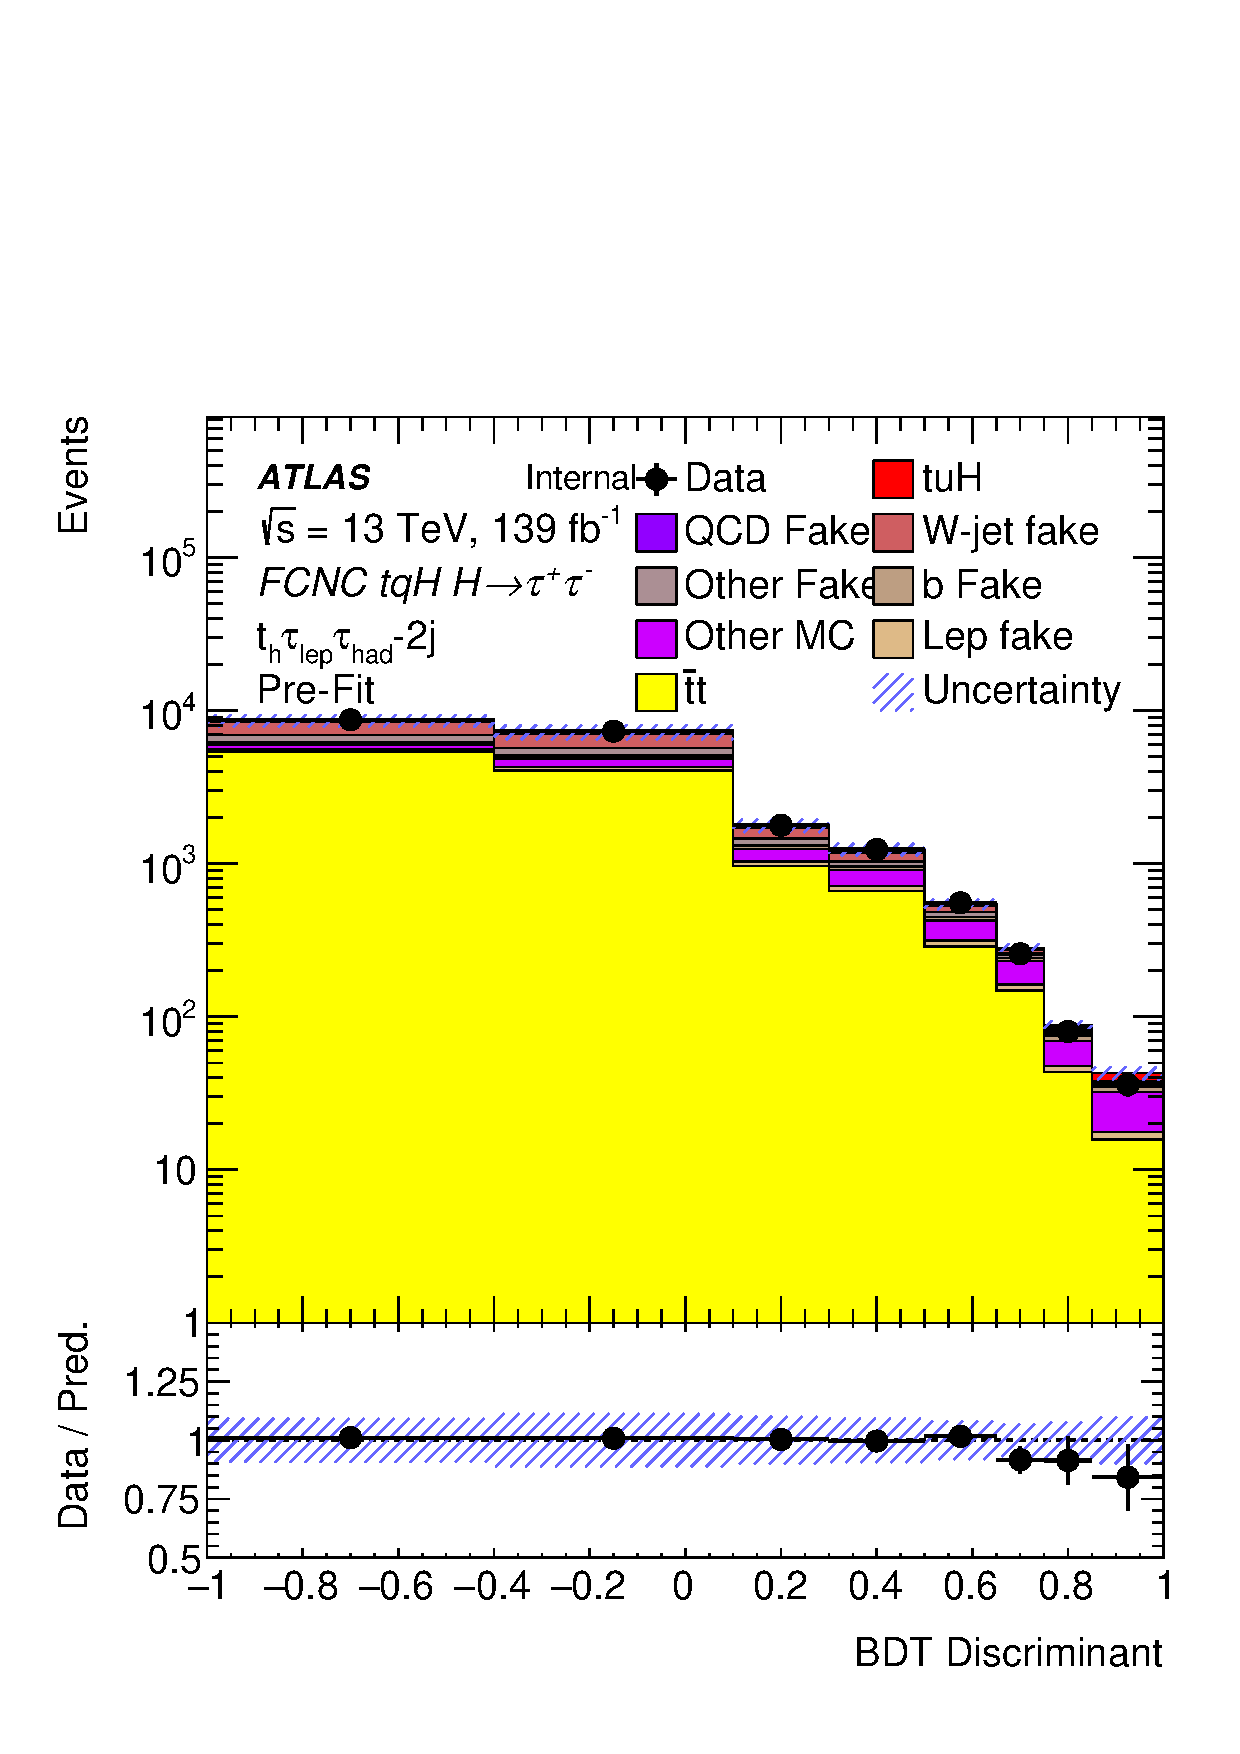
\includegraphics[width=0.45\textwidth]{\FCNCFigures/tthML/Limit/tuH_reg1l1tau1b2j_os.pdf}
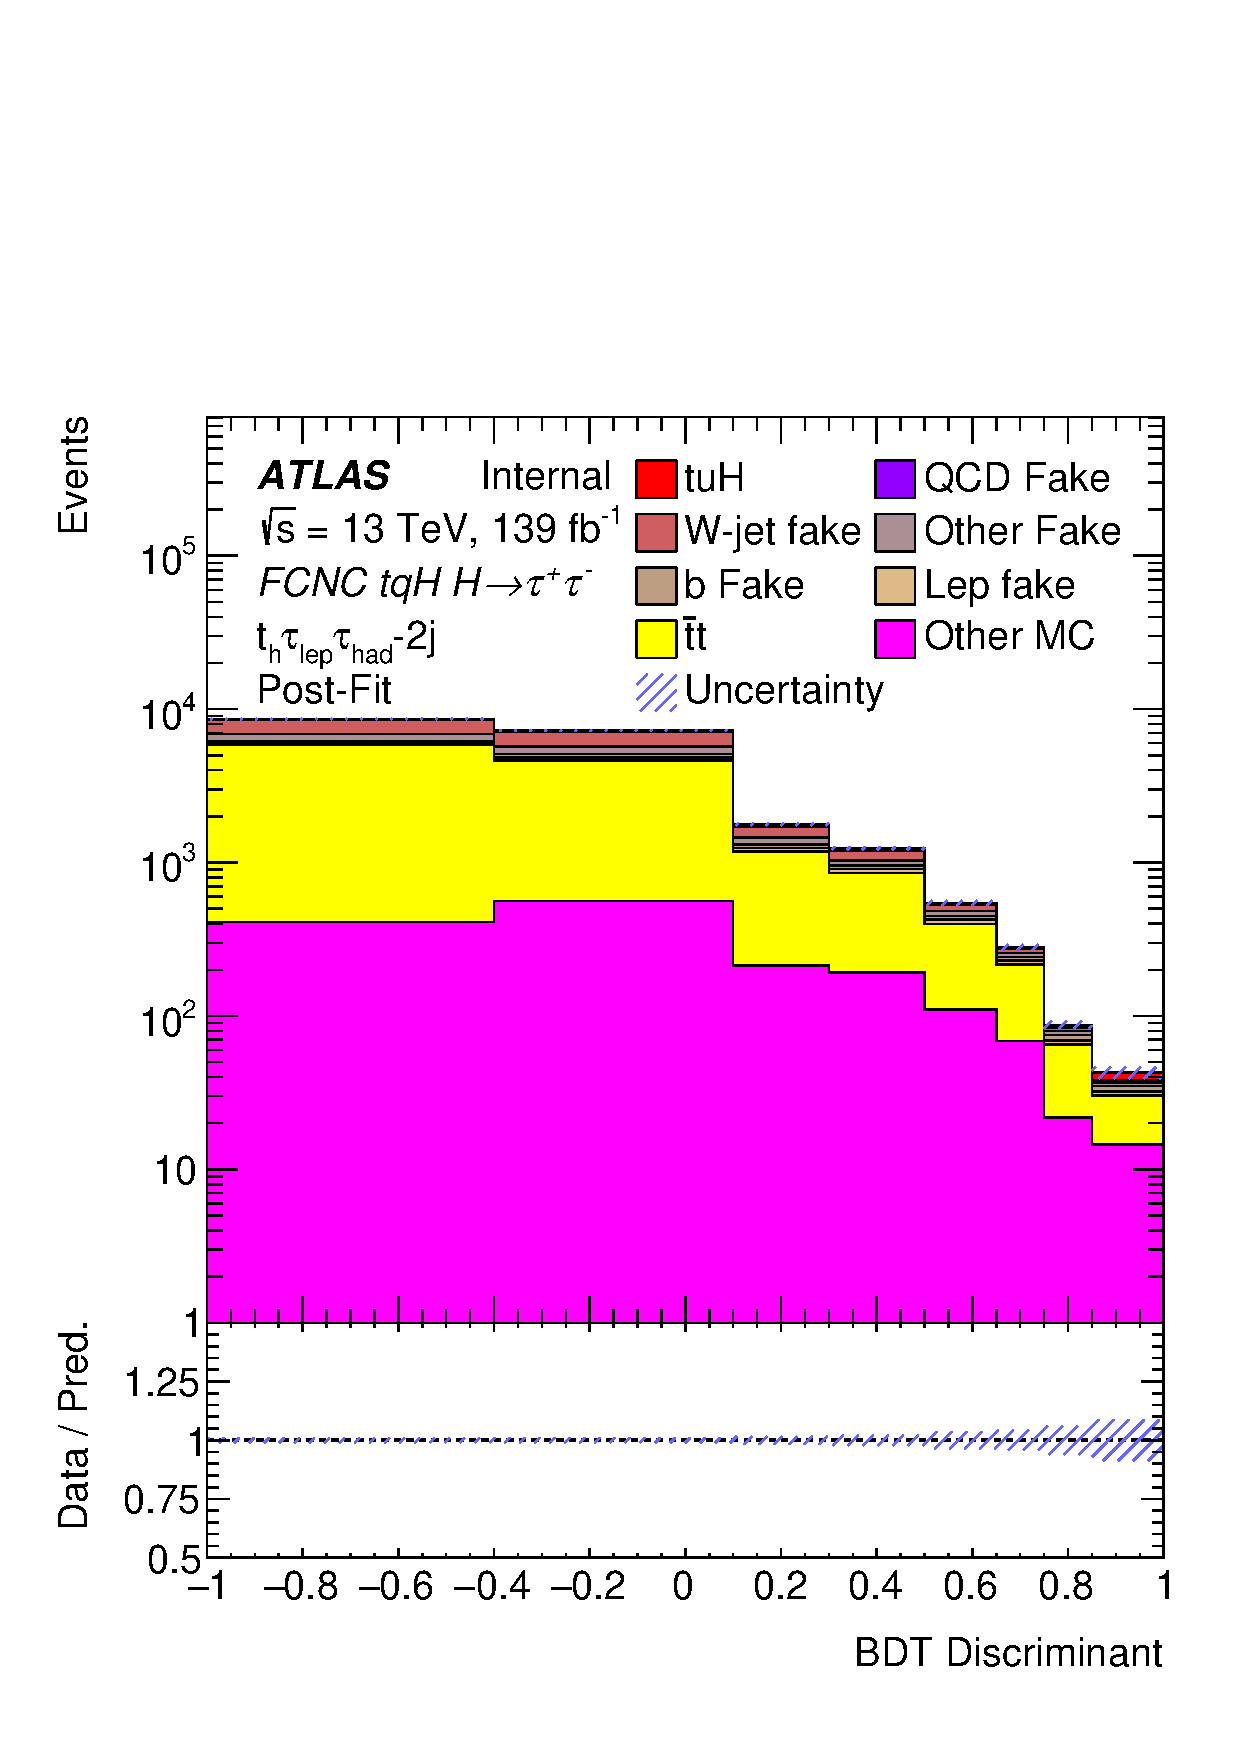
\includegraphics[width=0.45\textwidth]{\FCNCFigures/tthML/Limit/tuH_reg1l1tau1b2j_os_postFit.pdf}\\
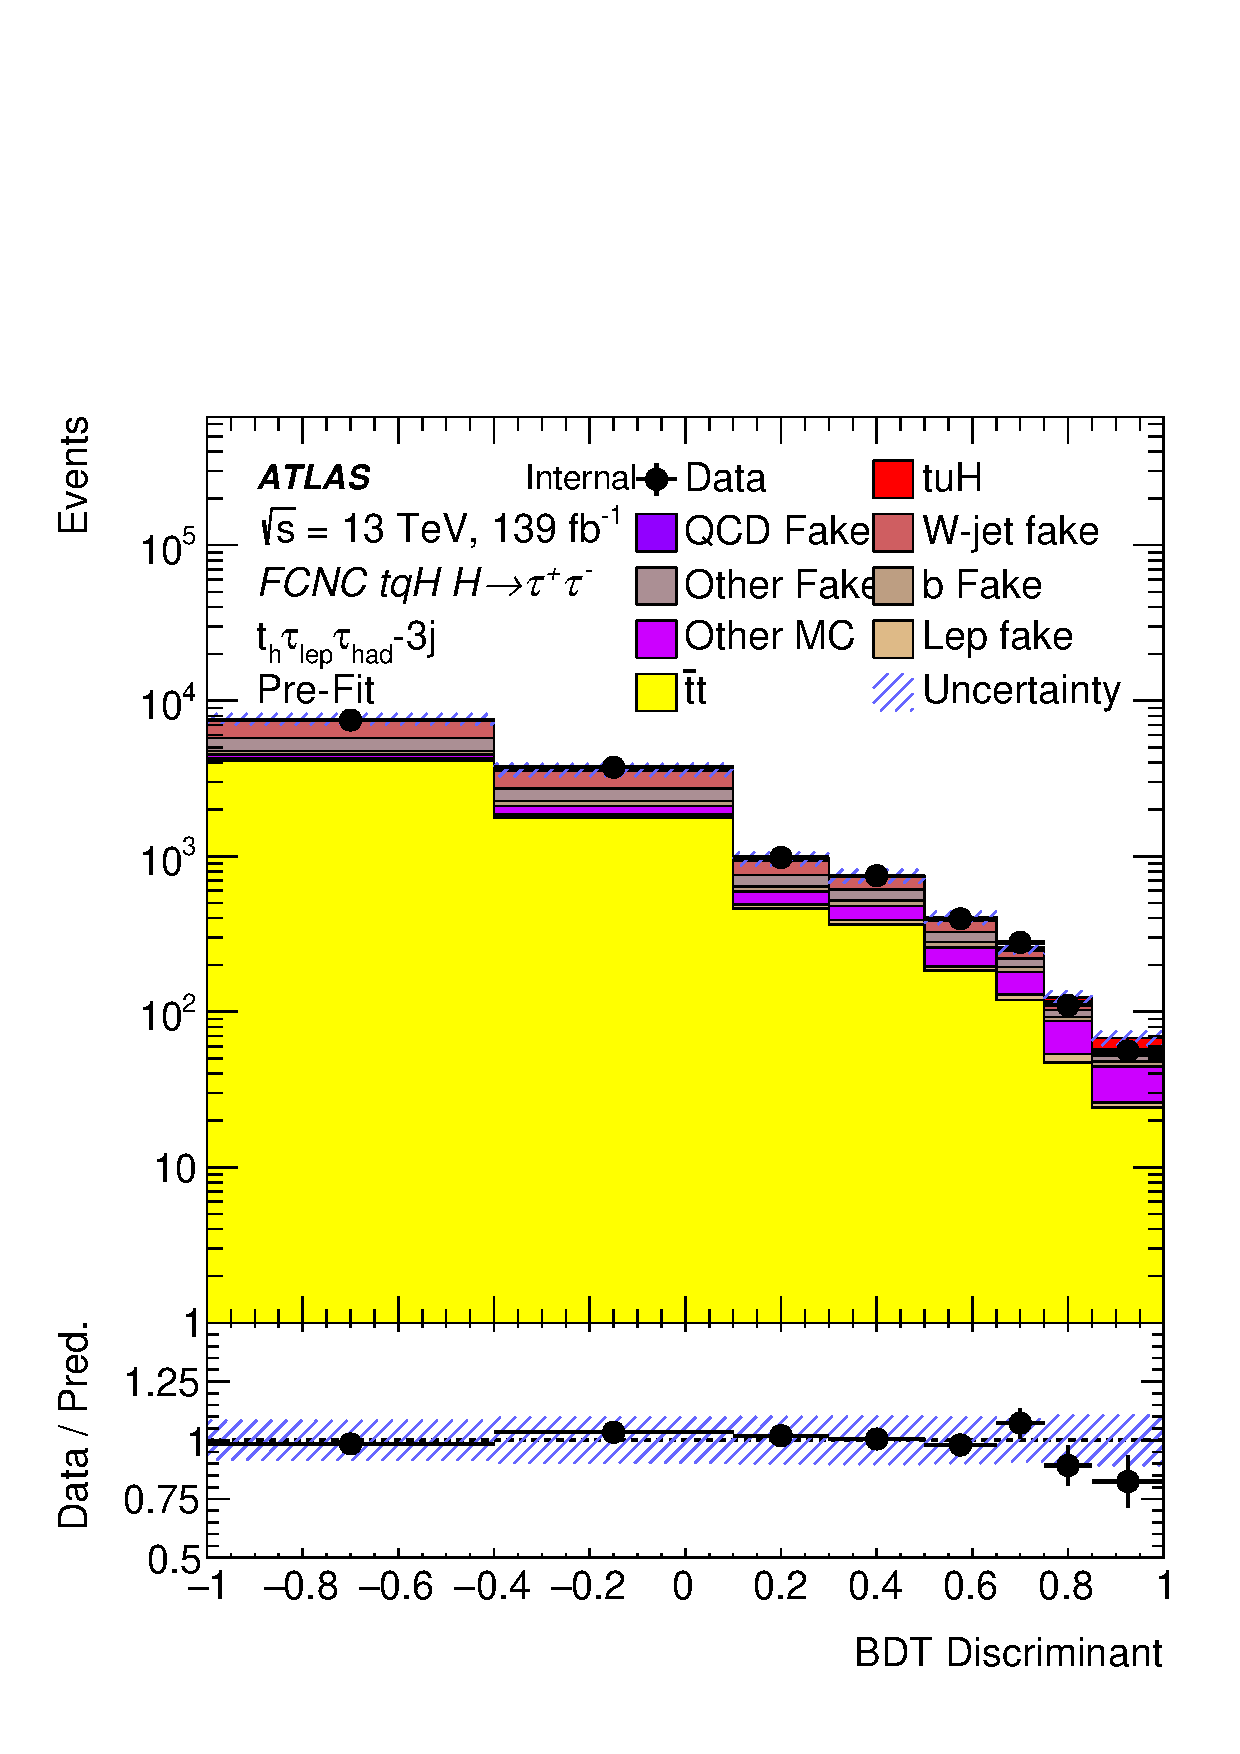
\includegraphics[width=0.45\textwidth]{\FCNCFigures/tthML/Limit/tuH_reg1l1tau1b3j_os.pdf}
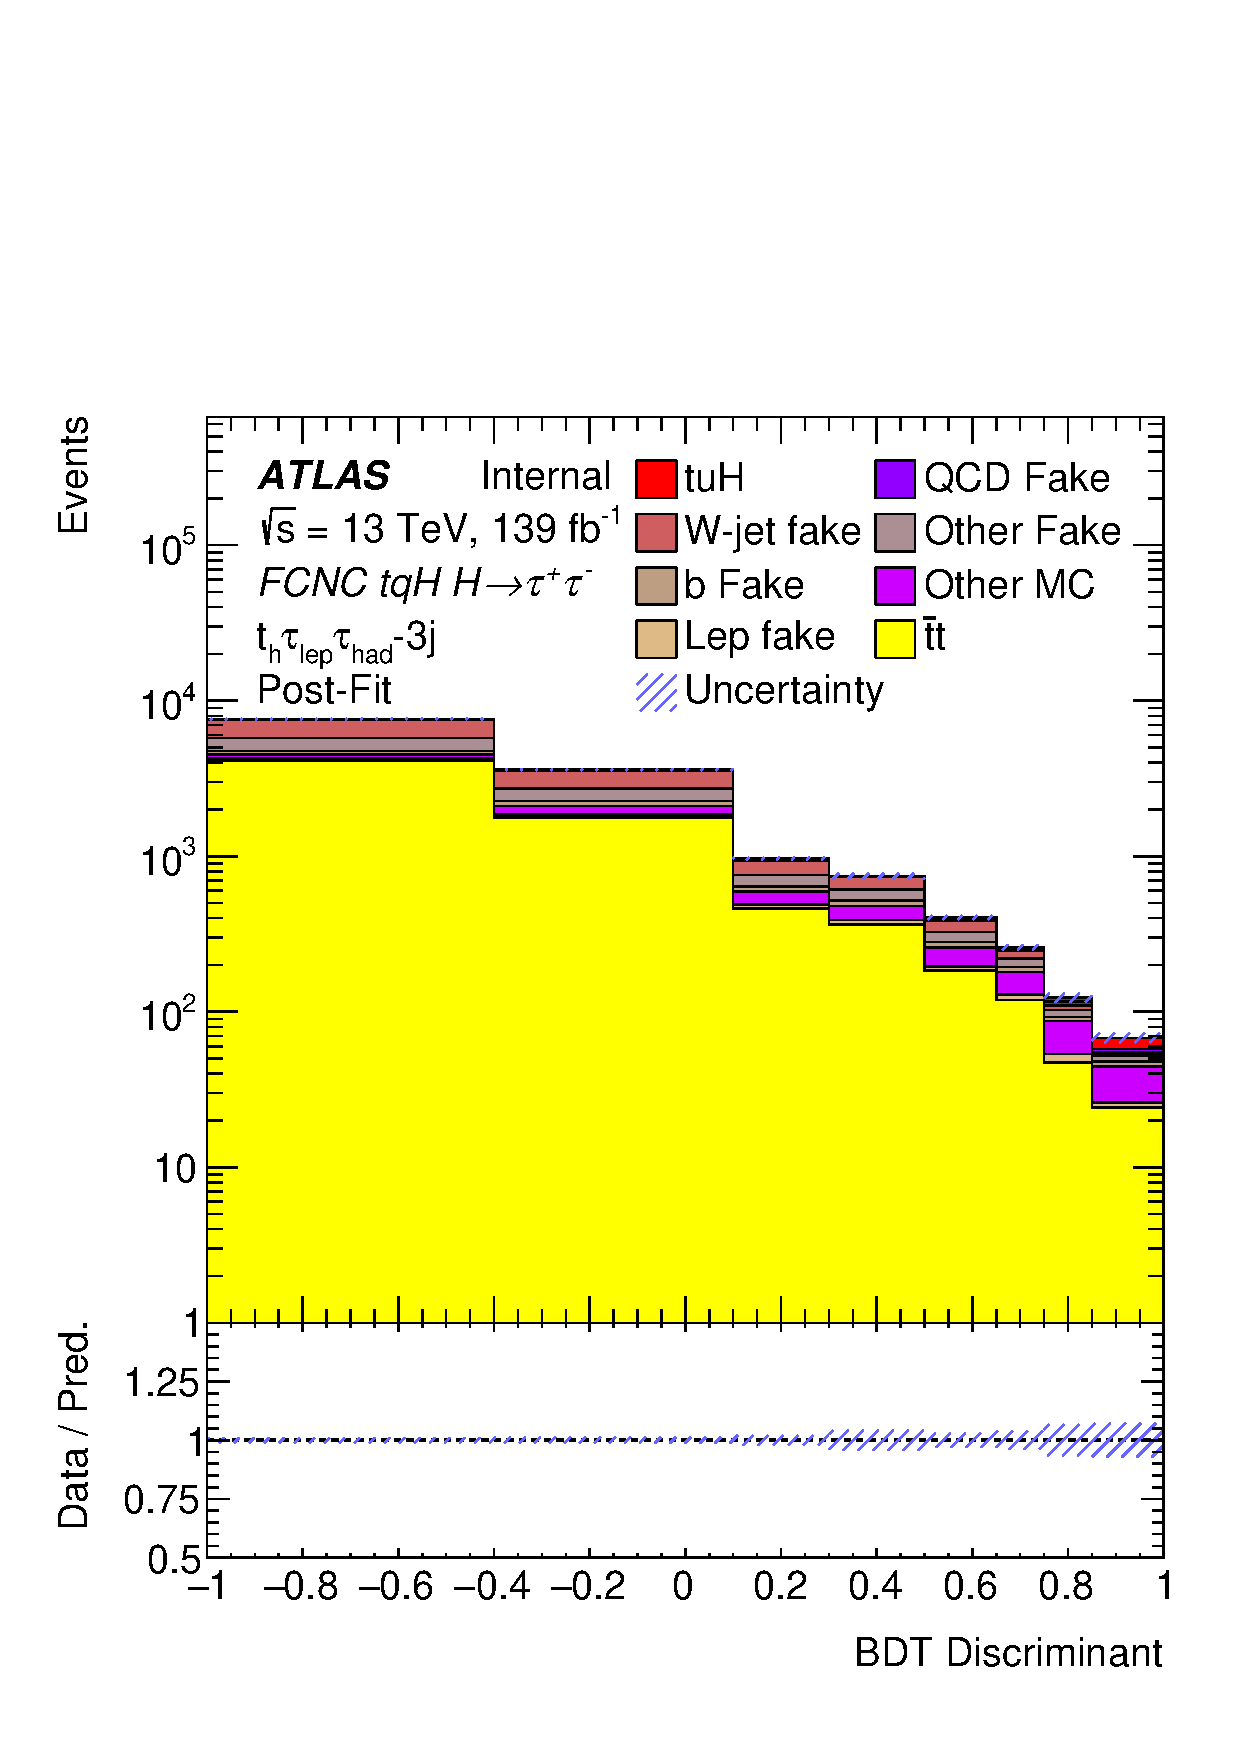
\includegraphics[width=0.45\textwidth]{\FCNCFigures/tthML/Limit/tuH_reg1l1tau1b3j_os_postFit.pdf}\\

\caption{ 两个$\tlhad$信号区拟合之前(左图)和使用赝数据拟合之后(右图)的BDT分数分布。}
\label{fig:tthML_trexPrefit}
\end{figure}

\begin{figure}[H]
\centering
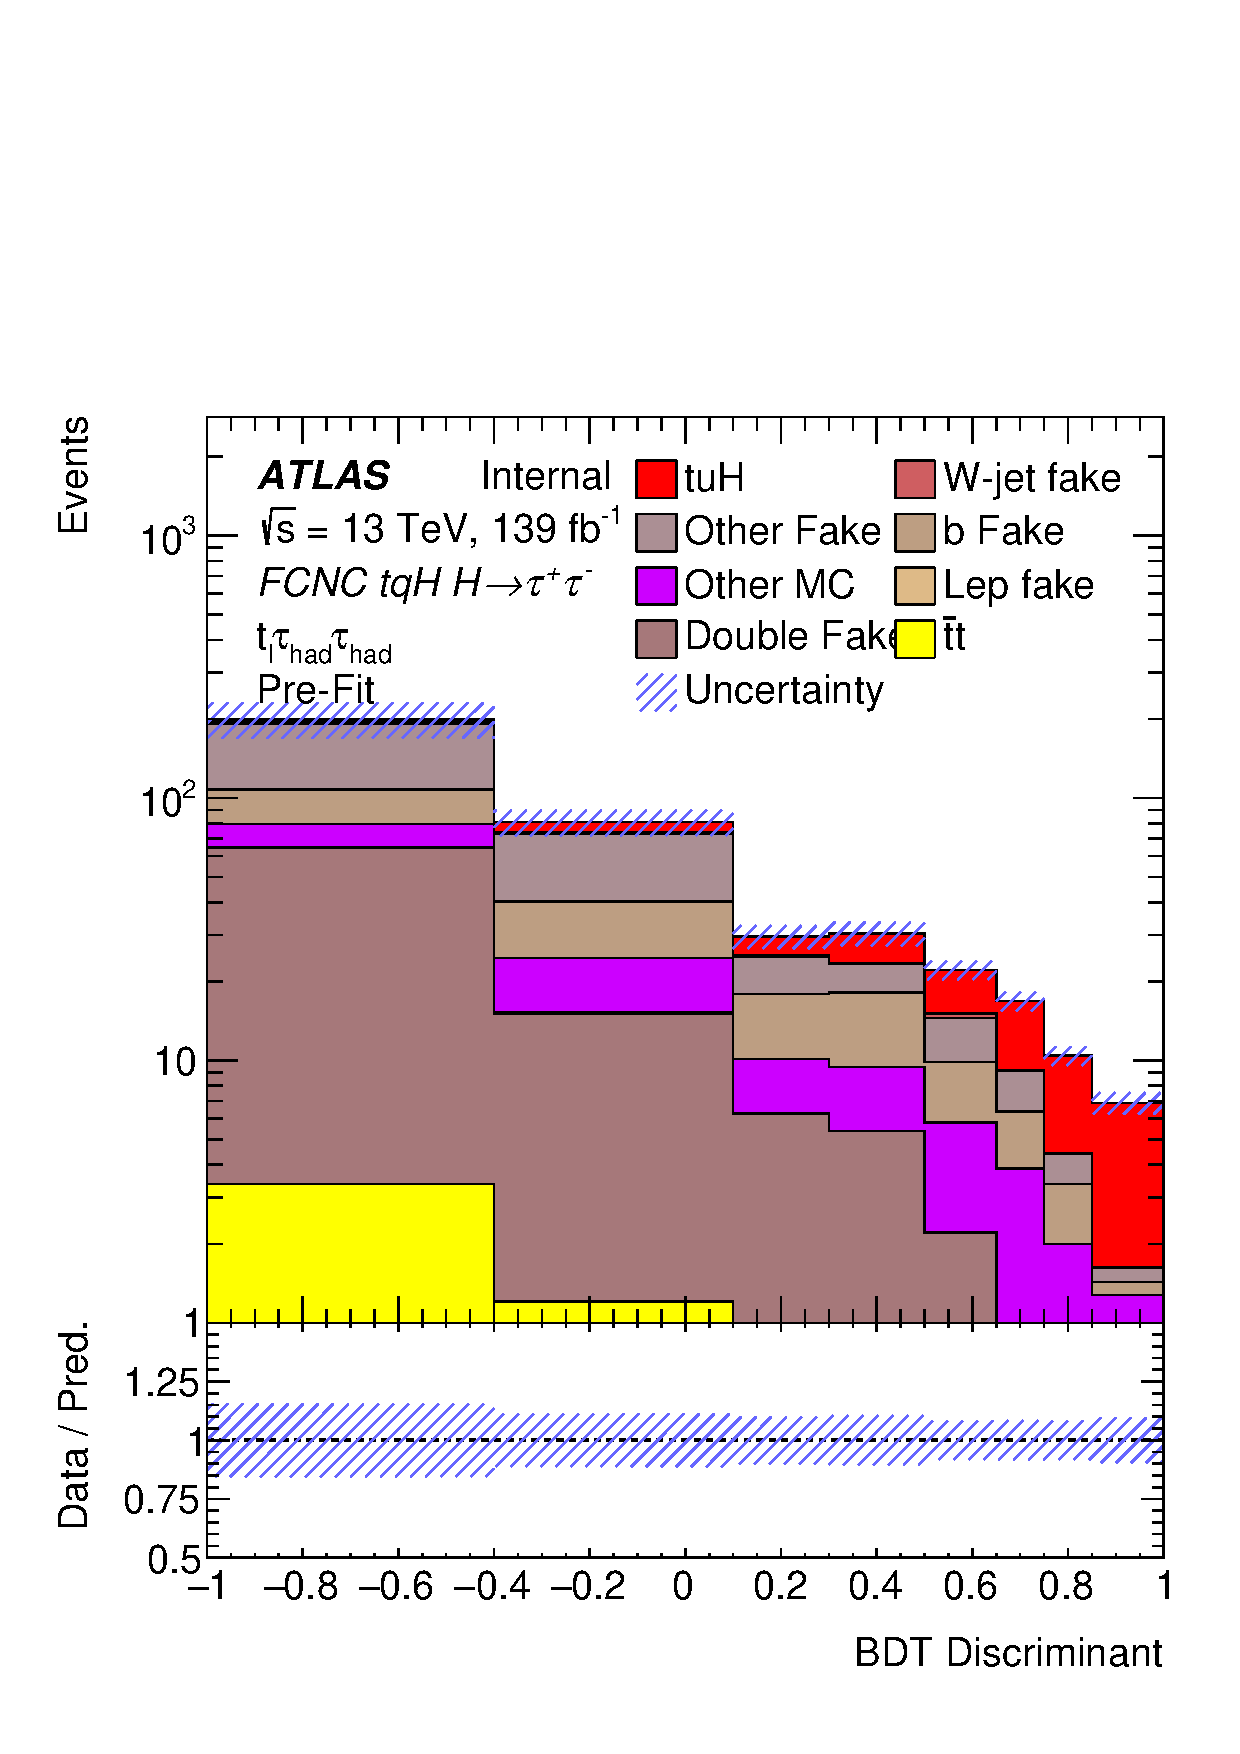
\includegraphics[width=0.45\textwidth]{\FCNCFigures/tthML/Limit/tuH_reg1l2tau1bnj_os.pdf}
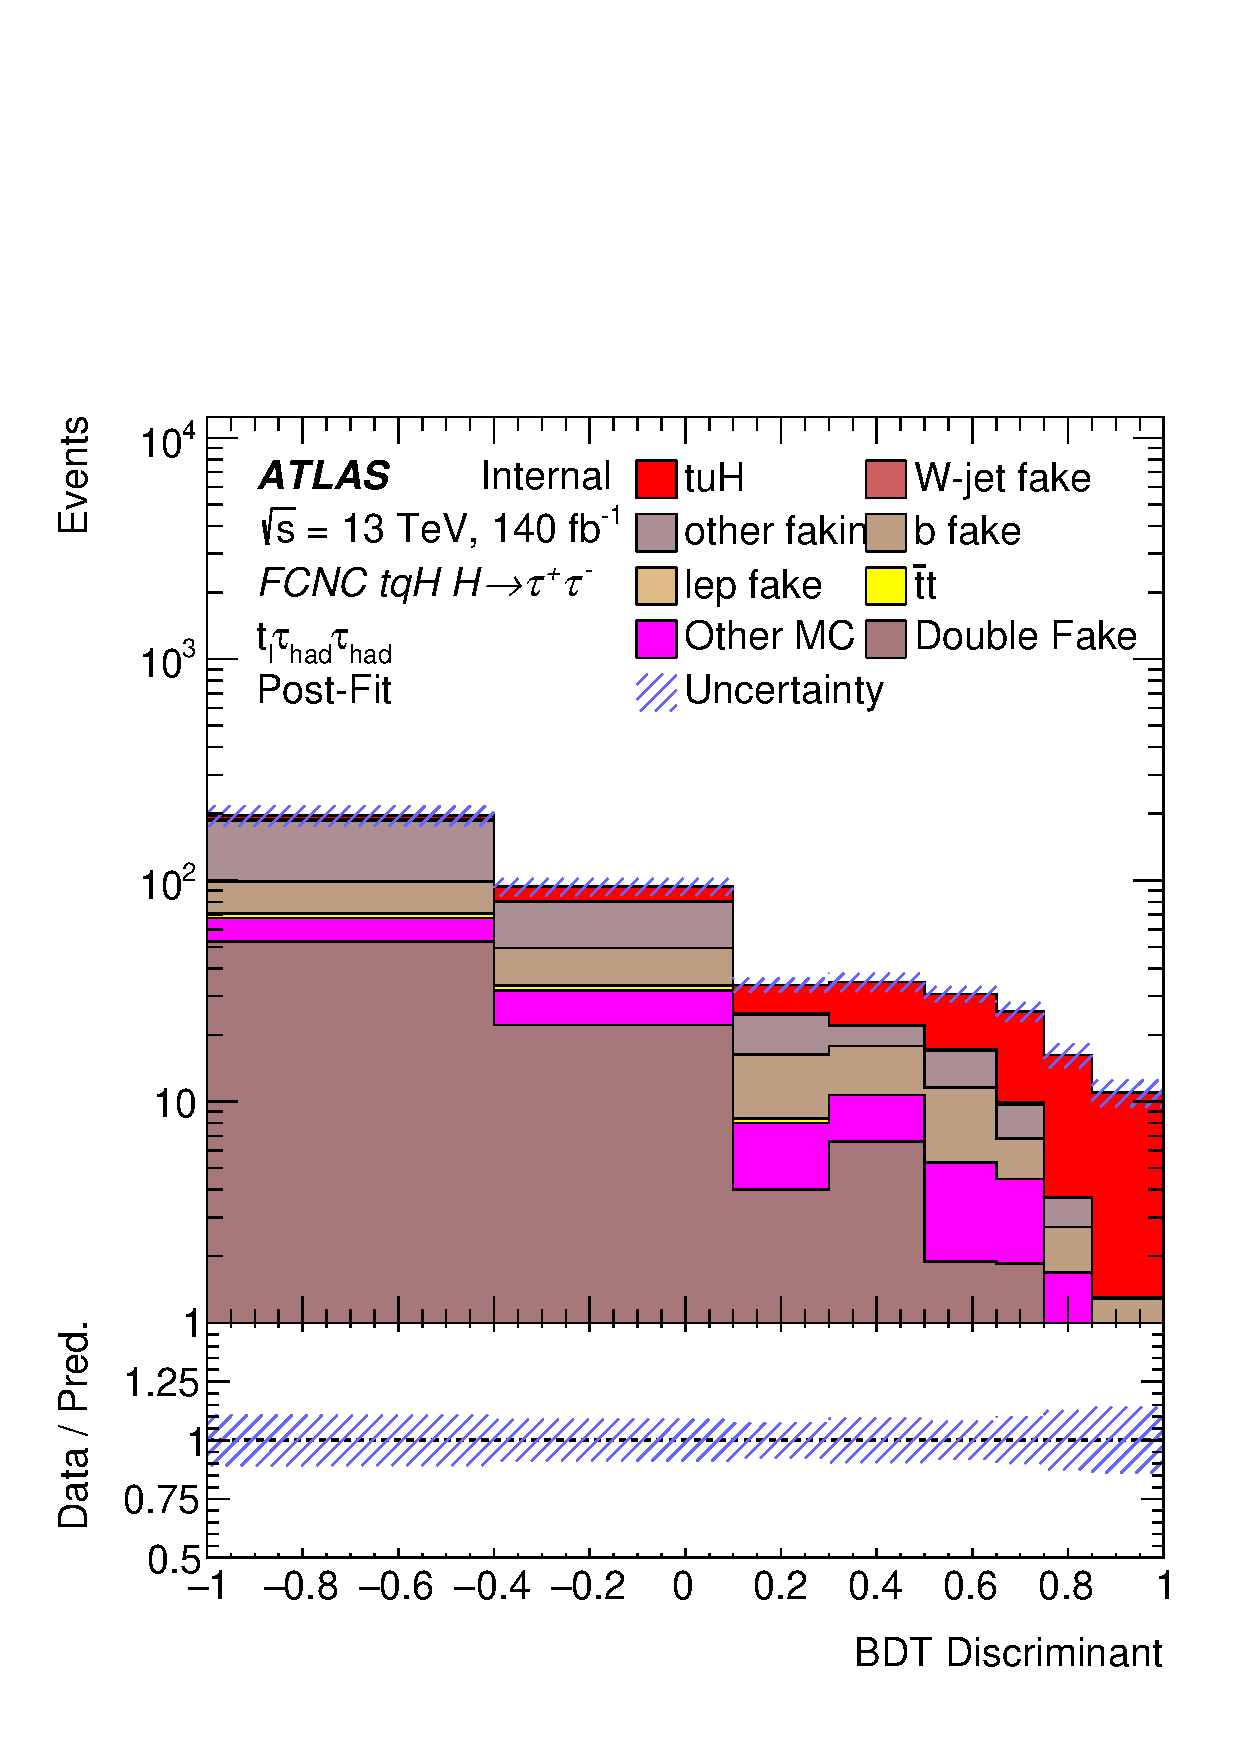
\includegraphics[width=0.45\textwidth]{\FCNCFigures/tthML/Limit/tuH_reg1l2tau1bnj_os_postFit.pdf}\\
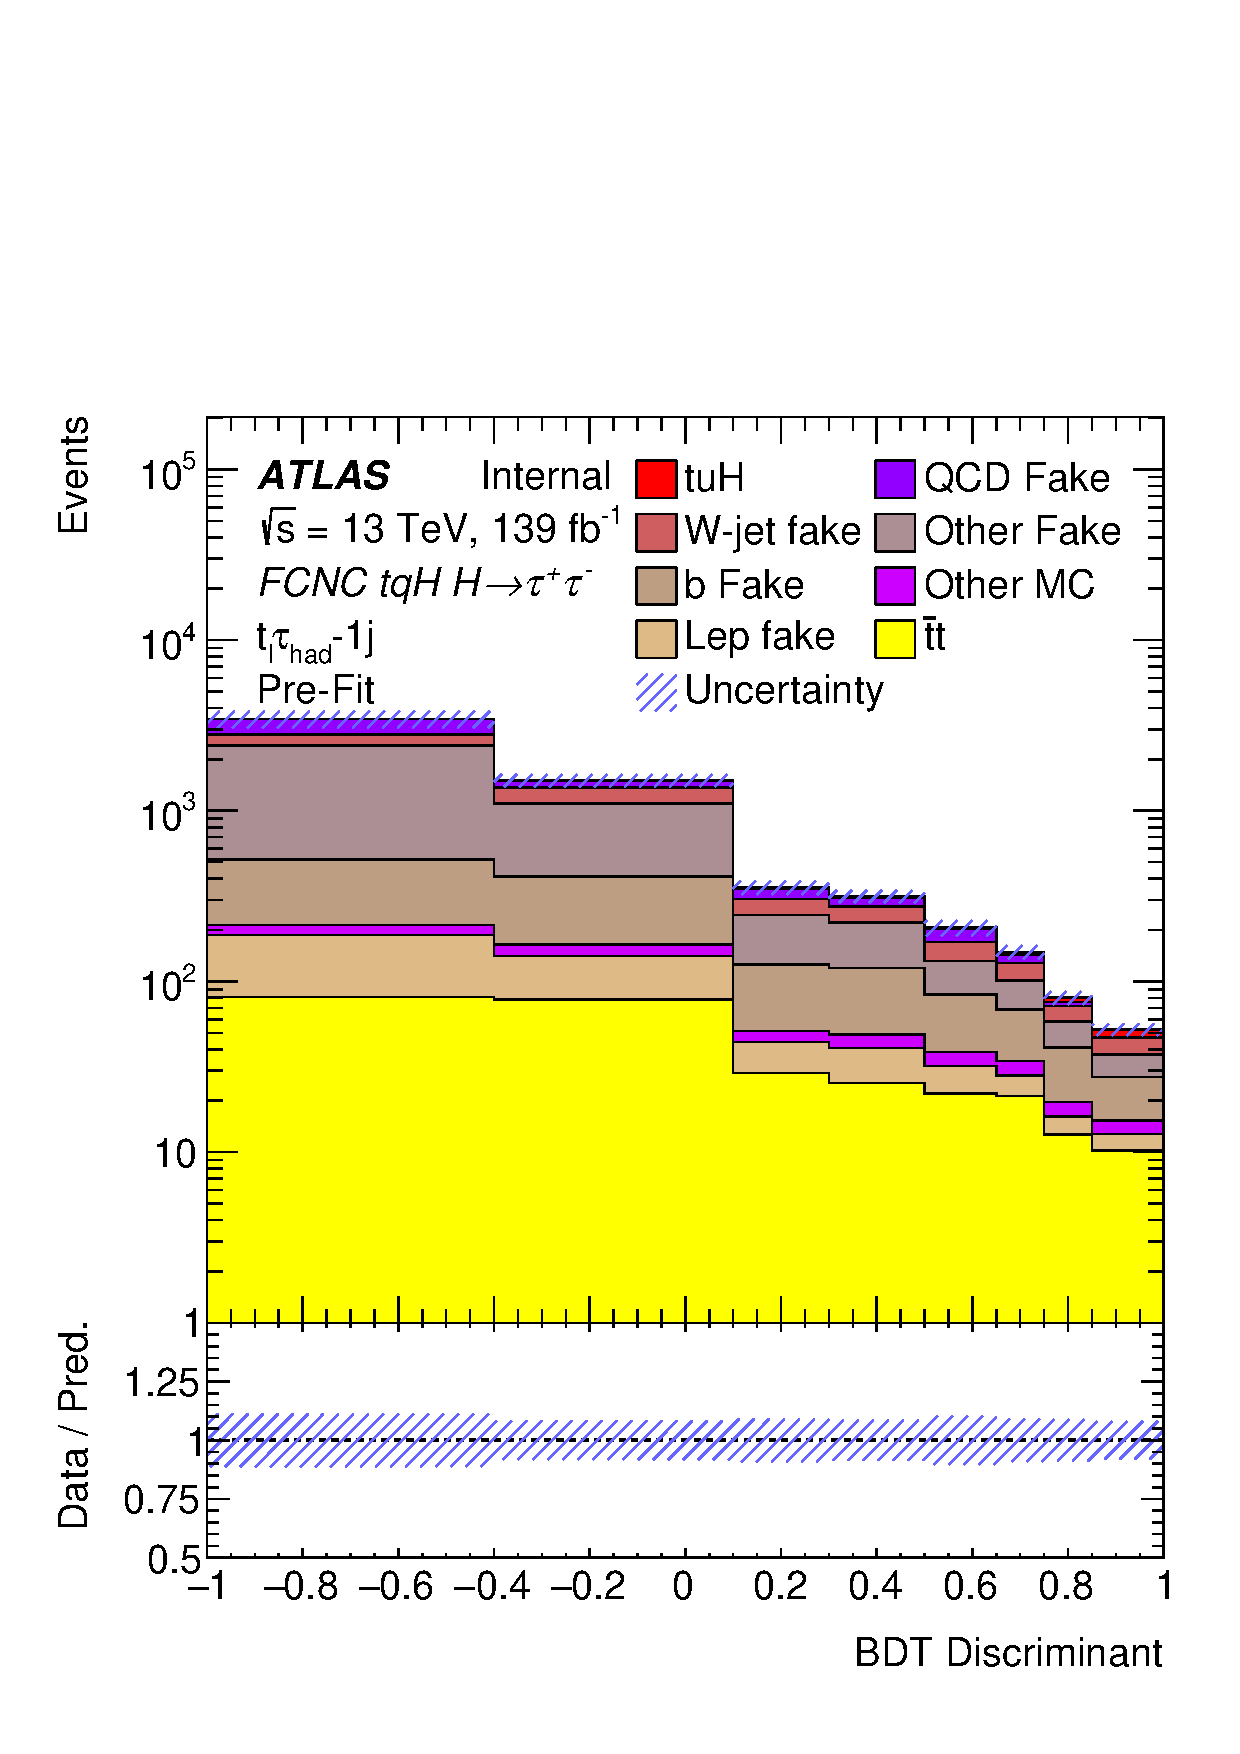
\includegraphics[width=0.45\textwidth]{\FCNCFigures/tthML/Limit/tuH_reg1l1tau1b1j_ss.pdf}
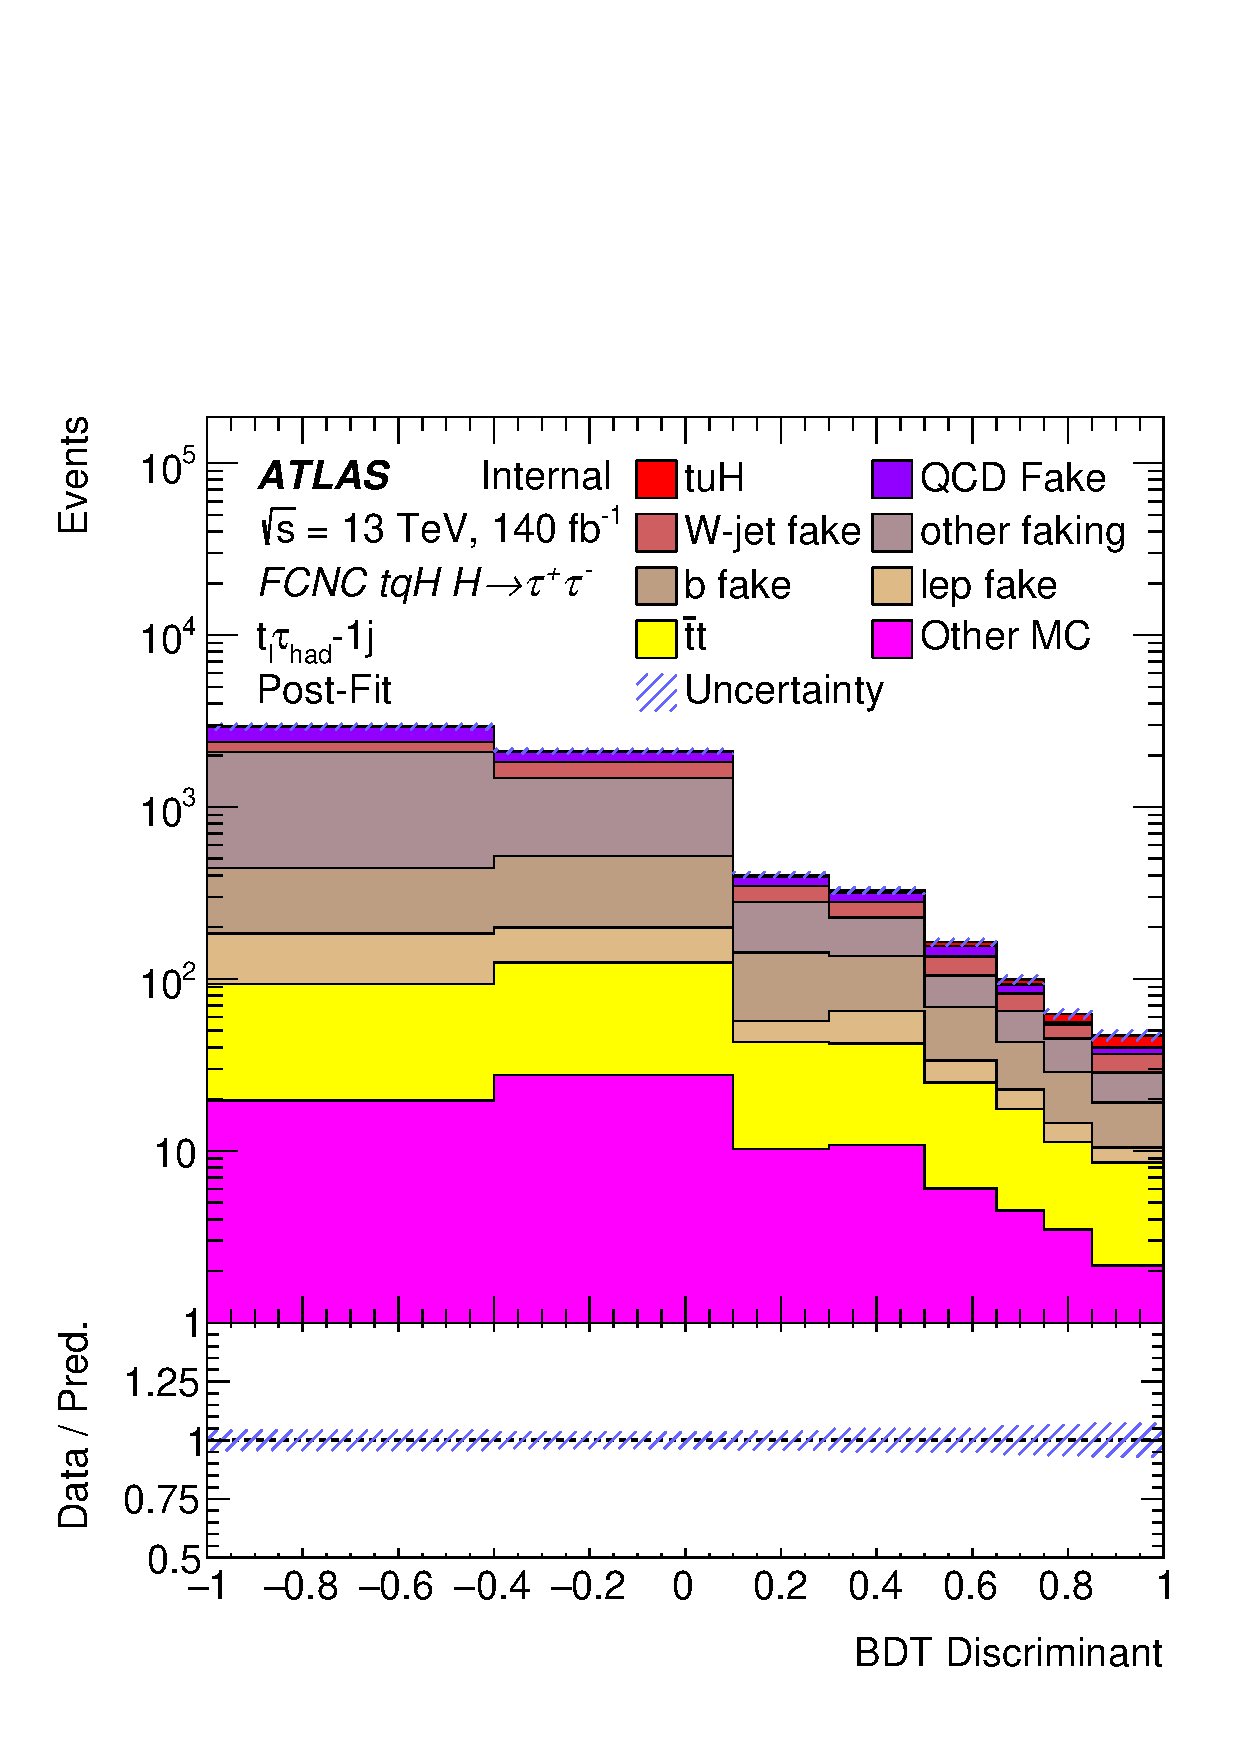
\includegraphics[width=0.45\textwidth]{\FCNCFigures/tthML/Limit/tuH_reg1l1tau1b1j_ss_postFit.pdf}\\
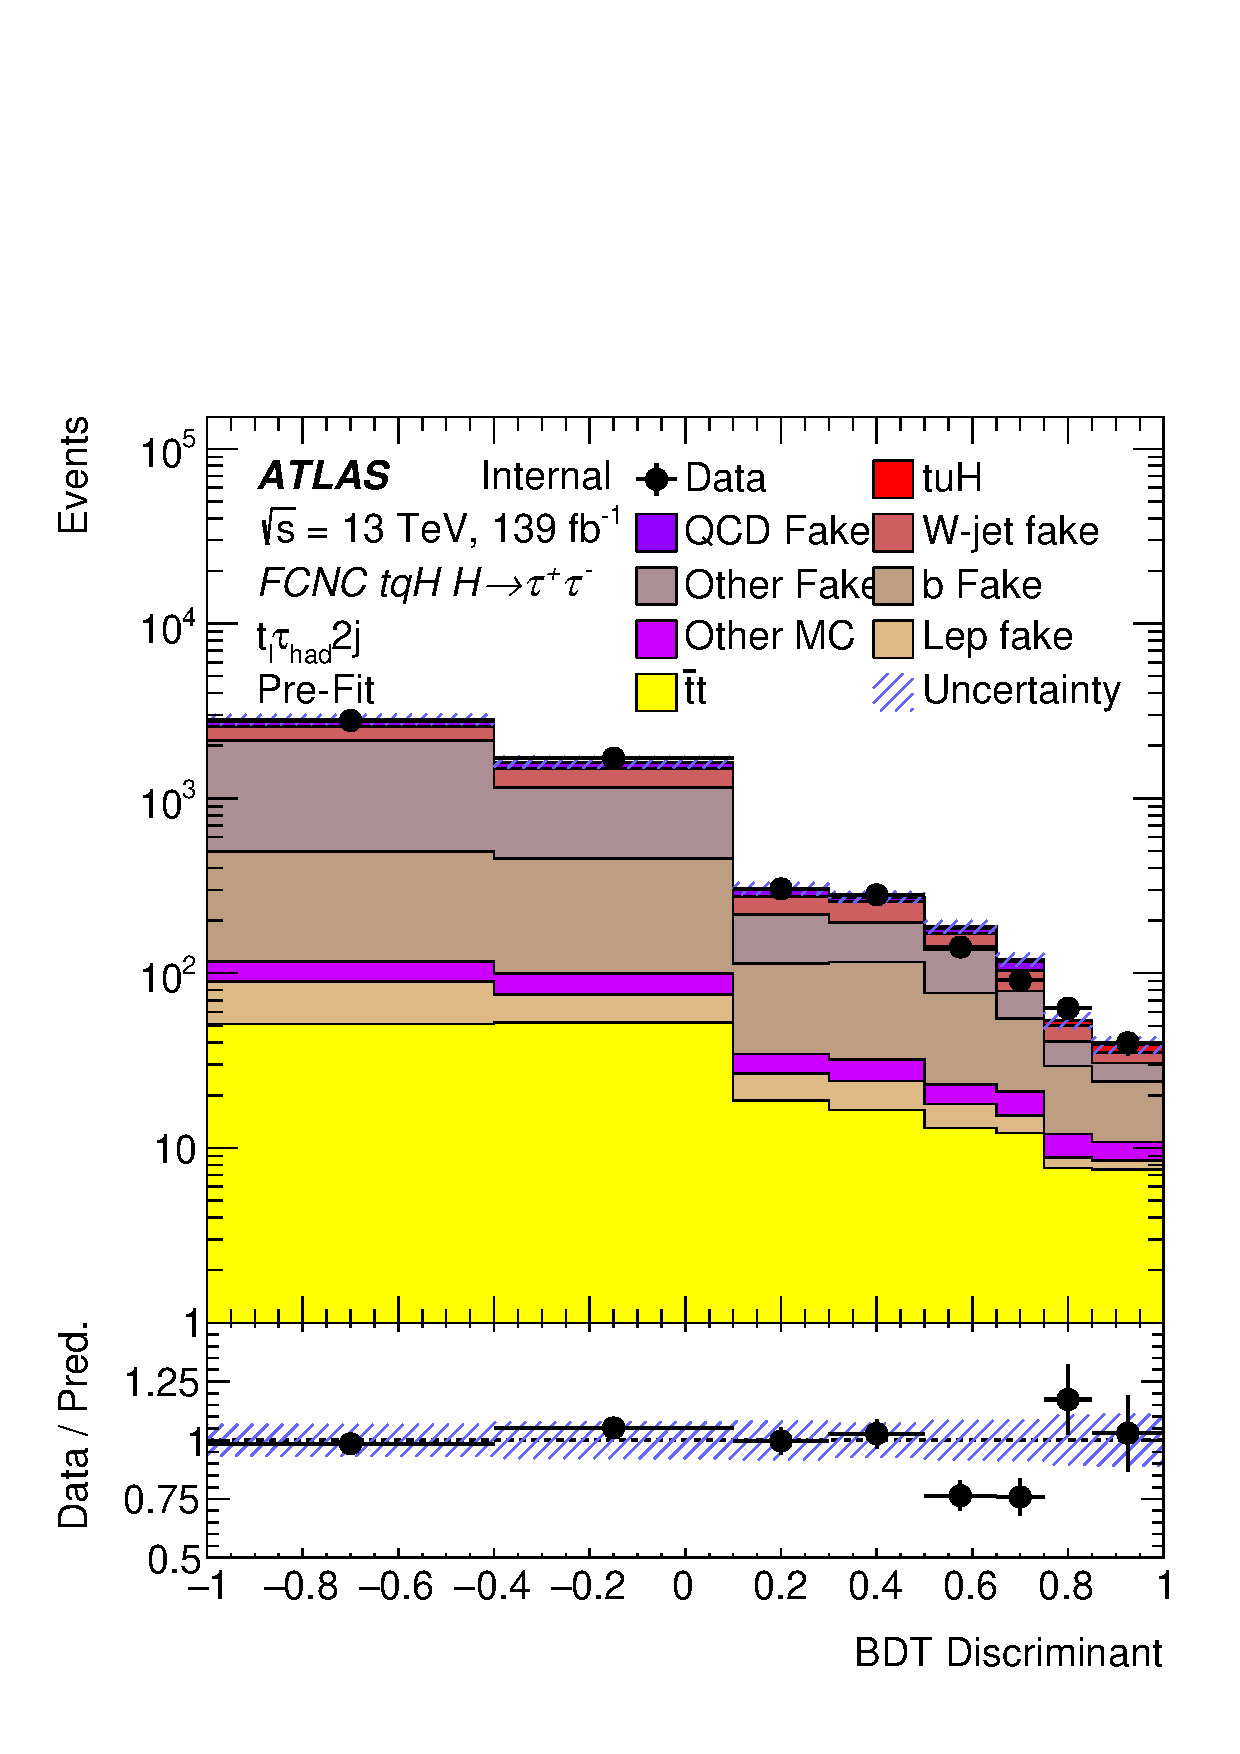
\includegraphics[width=0.45\textwidth]{\FCNCFigures/tthML/Limit/tuH_reg1l1tau1b2j_ss.pdf}
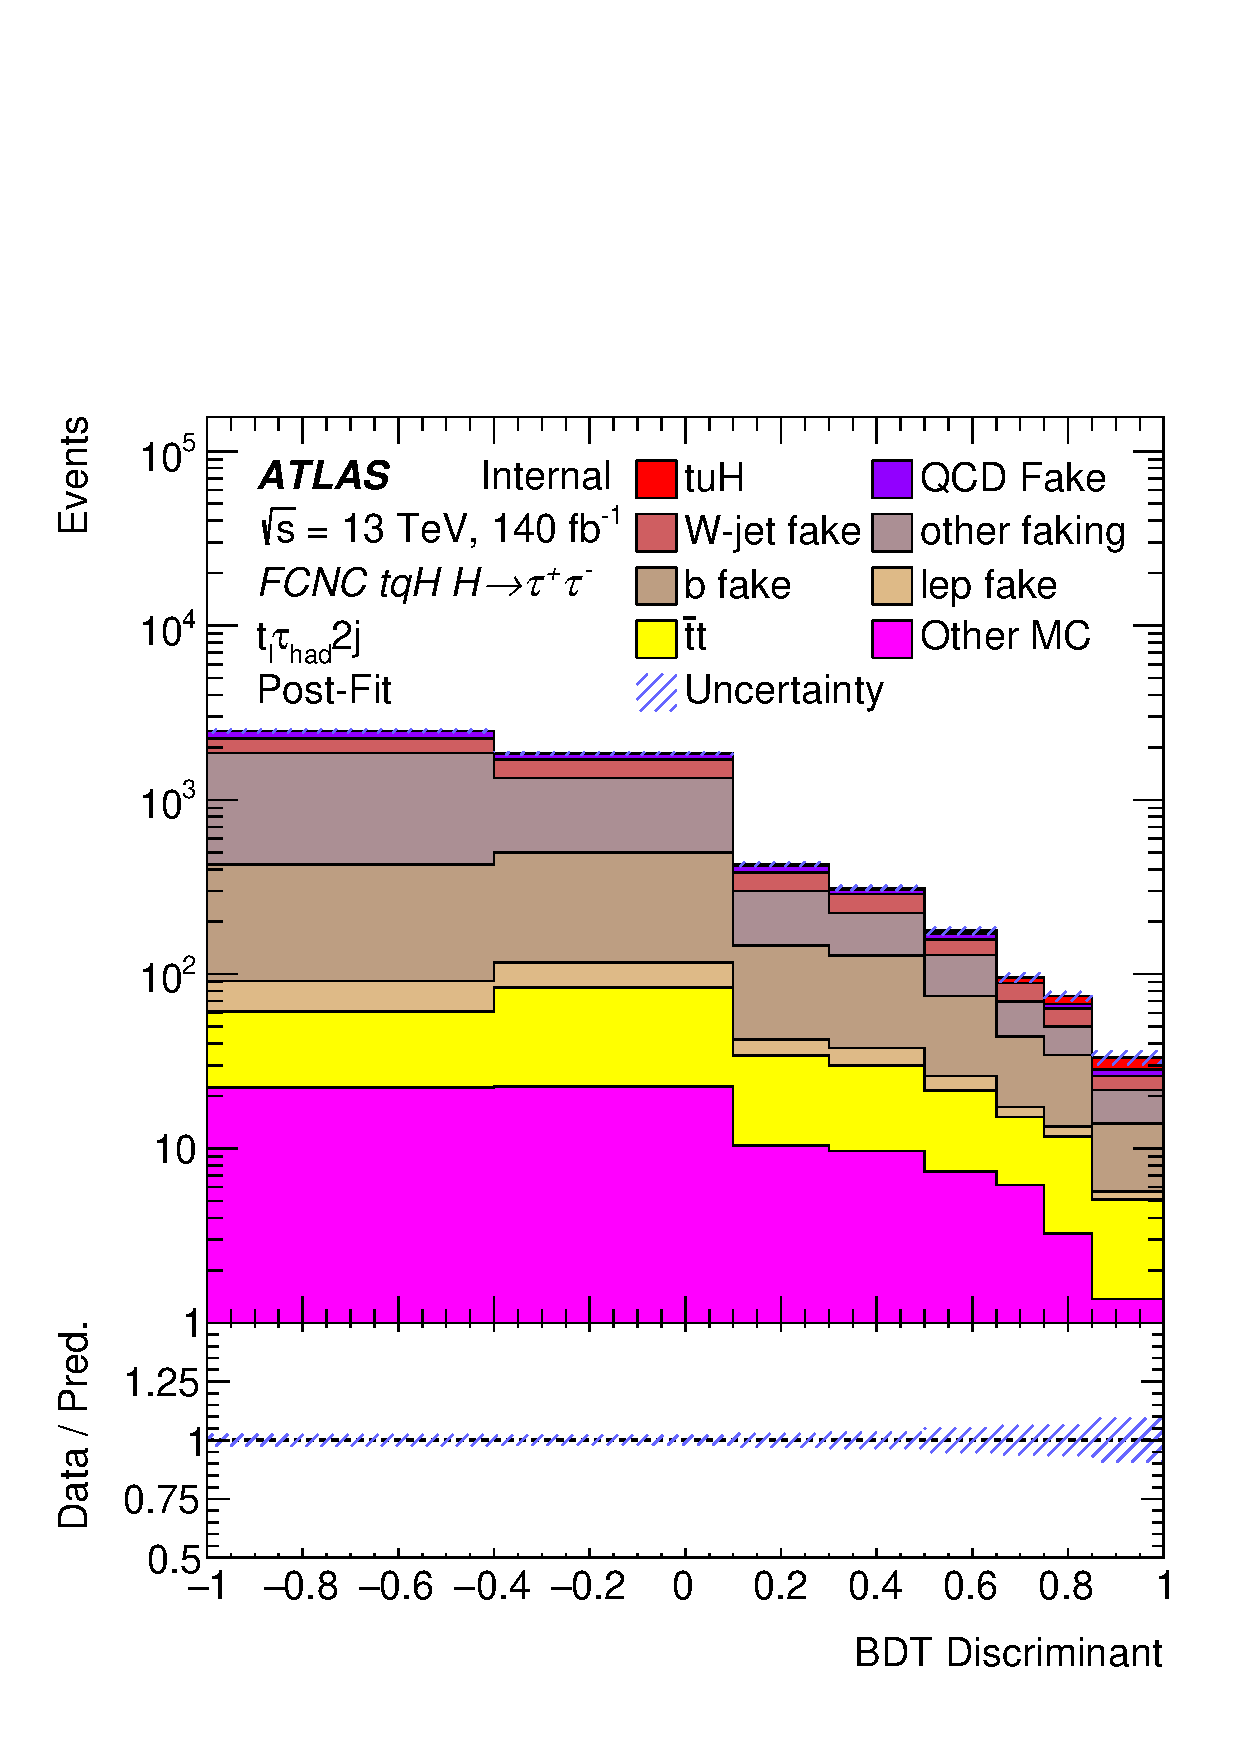
\includegraphics[width=0.45\textwidth]{\FCNCFigures/tthML/Limit/tuH_reg1l1tau1b2j_ss_postFit.pdf}\\

\caption{ $l\thadhad$和两个$l\tauhad$信号区拟合之前(左图)和使用赝数据拟合之后(右图)的BDT分数分布。}
\label{fig:tthML_trexPrefit_1}
\end{figure}
